\documentclass[conference]{IEEEtran}
\IEEEoverridecommandlockouts
% The preceding line is only needed to identify funding in the first footnote. If that is unneeded, please comment it out.
\usepackage{cite}
\usepackage{amsmath,amssymb,amsfonts}
\usepackage{algorithmic}
\usepackage{graphicx}
\usepackage{textcomp}
\usepackage{lipsum}
\usepackage{xcolor}
\usepackage{todonotes}
\usepackage{longtable}
\usepackage{float}

\usepackage{tikz}
\usepackage{pgfplots}
\usepgfplotslibrary{polar}


\def\BibTeX{{\rm B\kern-.05em{\sc i\kern-.025em b}\kern-.08em
    T\kern-.1667em\lower.7ex\hbox{E}\kern-.125emX}}
\begin{document}

\title{Analysis of Data Quality Management Maturity Level at PT Bank XYZ\\
% {\footnotesize \textsuperscript{*}Note: Sub-titles are not captured in Xplore and
% should not be used}
% \thanks{Identify applicable funding agency here. If none, delete this.}
}

\author{\IEEEauthorblockN{1\textsuperscript{st} Filzahanti Nuha Ramadhani}
\IEEEauthorblockA{
\textit{Fakultas Ilmu Komputer} \\
\textit{Universitas Indonesia}\\
Jakarta, Indonesia \\
filzahanti.nuha31@ui.ac.id}

\and
\IEEEauthorblockN{2\textsuperscript{rd} Jon Felix Germinian}
\IEEEauthorblockA{
\textit{Fakultas Ilmu Komputer} \\
\textit{Universitas Indonesia}\\
Jakarta, Indonesia \\
jon.felix@ui.ac.id}

\and
\IEEEauthorblockN{3\textsuperscript{nd} Samuel Mulatua Jeremy Nainggolan}
\IEEEauthorblockA{
\textit{Fakultas Ilmu Komputer} \\
\textit{Universitas Indonesia}\\
Jakarta, Indonesia \\
samuel.mulatua41@ui.ac.id}
}

\maketitle

\begin{abstract}
In the banking industry, high-quality data is essential for operational efficiency, regulatory compliance, and strategic decision-making. Understanding the maturity level of Data Quality Management (DQM) is crucial for PT Bank XYZ to identify gaps and uncover opportunities for improvement. Poor data quality can lead to significant risks, including inaccurate reporting, flawed decision-making, financial losses, and regulatory penalties. This study evaluates the DQM maturity at PT Bank XYZ using David Loshin’s Data Quality Framework and the Data Management Body of Knowledge (DMBOK) guidelines.
The research involves comprehensive interviews with key stakeholders to assess the bank's performance across eight DQM components, including governance, standards, and technology. The findings reveal an average maturity level of 2.04, classified as "Repeatable." While PT Bank XYZ demonstrates strength in data standard aspect, it struggles with deficiencies in data governance, quality protocols, and the implementation of advanced data technologies. These gaps hinder the bank’s ability to fully leverage its data assets for strategic growth and regulatory compliance.
To address these challenges, the study provides actionable recommendations aimed at enhancing DQM practices. By adopting these strategies, PT Bank XYZ can improve its data quality framework, reduce risks, and achieve a more sustainable competitive advantage.
\end{abstract}

\begin{IEEEkeywords}
data quality management; maturity model; maturity level; banking data
\end{IEEEkeywords}

\listoftodos

\section{Introduction}
Organizations today generate and manage data from a variety of sources, requiring robust systems to handle customer profiles, financial transactions, account management, and credit applications. Managing data quality (DQM) has become a critical focus for organizations, particularly in the banking sector, where accurate and reliable data serves as a cornerstone for operational efficiency and strategic growth. Poor data quality can lead to inaccuracies that hinder decision-making, such as selecting optimal business locations, and can expose organizations to reputational and financial risks.

In the context of PT Bank XYZ, understanding the maturity level of Data Quality Management (DQM) is crucial to identify gaps and opportunities for improvement. The bank operates in a complex data ecosystem, integrating Core Banking Systems (CBS), Customer Relationship Management (CRM) platforms, and regulatory compliance tools. These systems demand high data quality to meet operational needs and comply with regulations, such as POJK No. 8/2023 on Anti-Money Laundering and Counter Terrorism Financing.

To address these challenges, this paper explores the data quality maturity level of data quality management at PT XYZ and outlines strategies to enhance its governance framework. The study emphasizes the need for a holistic approach to data integration, quality monitoring, and regulatory compliance to ensure sustainable growth and resilience in the face of increasing data demands.

The study is guided by the following research questions:
\begin{enumerate}
    \item What is the current maturity level of data quality management at PT XYZ?
    \item How can PT XYZ improve its data quality management practices to address regulatory, operational, and strategic risks?
\end{enumerate}


\section{Related Works}

\todo{Tambah 2 studi disini}

This section explores three case studies highlighting diverse implementations of Data Quality Management (DQM) and Master Data Management (MDM). The first case study, as reported in \cite{dqmBPI2022}, focuses on PT BPI, where financial data quality management faces challenges due to errors, resulting in suboptimal decision-making in the public sector. The maturity level is at an initial stage, with reactive efforts managing structured financial data. The second case study, detailed in \cite{payani2023}, examines the National Remote Sensing Data Bank (BDPJN), which addresses the management of large volumes of satellite imagery data to support national planning. The organization demonstrates a maturity level ranging from defined to managed, handling unstructured remote sensing data. Lastly, \cite{hikmawati2021} discusses an MDM-based approach to improve data quality and governance, using the MD3M model to establish a "single source of truth" for transactional, inventory, and employee data. This study reflects a higher maturity level with a focus on consistent management of broader datasets, including customer, supplier, and material data. These case studies underscore the importance of tailored DQM and MDM practices to address organizational needs and data characteristics.


\section{Literature Review}

\subsection{Data Quality}

Data quality is essential for maintaining the usability, reliability, and trustworthiness of data. The Data Management Association International (DAMA) has identified six key dimensions of data quality that are widely acknowledged \cite{DAMA_2013} and applied across various fields \cite{wahyudi2023data, kiran2024addressing, antonio2024data}:  

\begin{itemize}
    \item \textbf{Completeness}: This dimension assesses whether all required data is present, ensuring no critical information is missing \cite{mahanti2019data}.
    \item \textbf{Uniqueness}: Ensures there is no redundant or duplicate data within a dataset, improving the overall integrity \cite{sebastiancoleman2022meeting}.
    \item \textbf{Timeliness}: Evaluates whether the data is up-to-date and relevant at the time of use, crucial for dynamic and real-time decision-making \cite{mashoufi2023data}.
    \item \textbf{Validity}: Verifies that the data adheres to predefined formats, business rules, and constraints \cite{mcgilvray2021executing}.
    \item \textbf{Accuracy}: Measures whether the data accurately represents real-world values or concepts, ensuring trustworthiness \cite{west2021towards}.
    \item \textbf{Consistency}: Examines whether data values are aligned across multiple datasets or systems, preventing contradictions \cite{antonio2024data}.
\end{itemize}

These dimensions are foundational for establishing robust data governance and quality frameworks. For instance, studies such as \cite{wahyudi2023data} and \cite{kiran2024addressing} have demonstrated the application of these dimensions in various sectors, including healthcare, smart mobility, and financial institutions. Practical approaches to implementing these dimensions are also elaborated in works like \cite{sebastiancoleman2022meeting} and \cite{mahanti2019data}, making them essential for ensuring effective data management strategies.

\subsection{Data Quality Management}
Data quality management is a strategic approach aimed at preserving data quality by incorporating activities such as planning, execution, and control to assess and maintain high-quality data standards.

\subsubsection{Components of DQM}

DMBOK identifies critical components of DQM:
\begin{itemize}
    \item \textbf{Governance}: Establishing accountability structures for data quality.
    \item \textbf{Profiling and Cleansing}: Identifying and resolving quality issues.
    \item \textbf{Root Cause Analysis}: Addressing systemic issues that cause poor data quality.
    \item \textbf{Monitoring and Improvement}: Continuously assessing and enhancing quality metrics.
\end{itemize}

The DMBOK life cycle comprises six phases: planning, implementation, evaluation, monitoring, maintenance, and improvement. This iterative process ensures data quality aligns with organizational goals.

\subsubsection{Challenges in Data Quality Management}
DMBOK highlights several challenges:
\begin{itemize}
    \item \textbf{Data Silos}: Fragmented systems leading to inconsistent data.
    \item \textbf{Dynamic Data}: Increased volume and complexity in big data ecosystems.
    \item \textbf{Lack of Standards}: Disparate definitions of data quality across departments.
    \item \textbf{Human Error}: Manual interventions that introduce inaccuracies.
\end{itemize}


\subsection{Data Quality Maturity}

Managing data quality effectively requires aligning data quality practices with organizational activities \cite{loshin_dqi}. However, data management is often treated as secondary to functional needs, leading to siloed systems. A data quality maturity model, adapted from the Capability Maturity Model (CMM), helps organizations assess and improve their practices, moving from ad hoc processes to optimized systems.



% \subsection{Data Quality Maturity Level}


% Maturity are divided to 5 level \cite{loshin_dqi}:

% \begin{itemize}
%     \item \textbf{Initial}: Reactive and ad hoc processes; fixes focus on immediate issues without addressing root causes.
%     \item \textbf{Repeatable}: Basic governance and limited documentation; some replication of successful practices, but technology remains unstandardized.
%     \item \textbf{Defined}: Established governance policies, documented practices, and consistent organization-wide processes with defined accountability.
%     \item \textbf{Managed}: Integration of business impact analysis, measurable performance metrics, and proactive flaw detection.
%     \item \textbf{Optimized}: Continuous process improvement with dashboards and systemic quality enhancements through adaptive standards and strategies.
% \end{itemize}


\subsection{Data Quality Maturity Model}

The maturity model connects organizational data practices to higher levels of performance and quality by addressing key components of data management \cite{loshin_dqi}. 
% Organizational maturity in managing data quality is reflected in the following components:

% \begin{itemize}
%     \item \textbf{Data Quality Expectations}: Aligns understanding between IT and business to define and use data quality dimensions effectively.
%     \item \textbf{Policies}: Evolves from informal, undocumented approaches to fully integrated, auditable policies tied to business activities.
%     \item \textbf{Procedures}: High-performance organizations rely on well-defined processes and protocols to ensure information quality.
%     \item \textbf{Governance}: Develops through bottom-up information sharing and top-down formalization of responsibilities.
%     \item \textbf{Standards}: Maturity is reflected in how data standards are defined and implemented to ensure interoperability.
%     \item \textbf{Technology}: Shifts from tool acquisition to enterprise-wide, service-oriented approaches for data quality improvement.
%     \item \textbf{Performance Management}: Focuses on defining objectives, measuring conformance, and meeting performance goals.
% \end{itemize}


% First part of the table
\begin{table}[H]
\caption{Comparison of Maturity Models)}
\label{tab:comparison-dqm-part1}
\centering
\begin{tabular}{|p{1.5cm}|p{3cm}|p{3cm}|}
\hline
\textbf{References} & \textbf{Maturity Levels} & \textbf{Dimensions} \\ \hline
Loshin \cite{loshin_dqi} & Initial, Repeatable, Defined, Managed, Optimized & Data Quality Expectations, Dimensions of Data Quality, Policies, Procedures, Governance, Standards, Technology, Performance Management \\ \hline
Ryu, K-S et al \cite{ryu2006dqm} & Initial, Defined, Managed, Optimized & Total corporate integration point of view, Data structure quality management point of view, Maturity stages point of view \\ \hline
Kirikoglu \cite{kirikoglu2017dqm} & Person, dependent and basic, Policies, standards, and procedures, Defined and stable, Managed and standardized, Continues improvement & Disciplined process, Standard consistent process, Predictable process, Continuously improving process \\ \hline
Ismael, C et al \cite{ismael2003caldea} & Initial, Definition, Integration, Quantitative Management, Optimizing & Data acquisition processes, Data product manufacturing process, and Data maintenance process \\ \hline
\end{tabular}
\end{table}

% % Second part of the table
% \begin{table}[h!]
% \caption{Comparison of Maturity Models (Part 2)}
% \label{tab:comparison-dqm-part2}
% \centering
% \begin{tabular}{|p{1.5cm}|p{3cm}|p{3cm}|}
% \hline
% \textbf{References} & \textbf{Maturity Levels} & \textbf{Dimensions} \\ \hline

% \end{tabular}
% \end{table}

In this study, the author selected David Loshin's data quality maturity model. This model was chosen because its dimensions are comprehensive and more adaptable for application in various companies, including PT Bank XYZ, compared to other models.

\section{Research Method}

This research stage begins with problem identification by asking Director of Operations where the key issue is defined to guide the study. Next, a literature review is conducted to previous research on the topic. Following this, a research instrument is developed using DQ Framework by David Loshin \cite{loshin_dqi} as interview guides. After the data is collected, a data quality management maturity assessment is performed. Finally, based on the findings, a data quality improvement strategy is developed to enhance the quality and effectiveness of the data for future analysis based on the Data Quality Activities by DMBOK.
\begin{figure}[H]
\centerline{\includegraphics[width=0.4\textwidth]{figures/AlurPenelitian.png}}
\caption{Research Stages}
\label{fig:untuk di ref di dokumen}
\end{figure}

\subsection{Research Instruments}

In this study, the DQM maturity level characteristic matrix, derived from David Loshin’s Data Quality Framework (DQF) \cite{loshin_dqi} is used as the instrument. The matrix consists of a checklist containing 121 characteristics spread across 8 components defined in the DQF, as summarized in TABLE II. For each characteristic a score of 1 will be assigned if the organization has implemented it and a score of 0 if it has not. The checklist will serve as a guide for questioning interviewees about the organization’s data quality management processes. 
\begin{table}[H]
\caption{Table of Questionnaire Areas and Number of Questions}
\label{tab:questionnare-areas}
\centering
\begin{tabular}{|l|c|}
\hline
\textbf{Questionnaire Area} & \textbf{\#Question} \\
\hline
Data Quality Expectations & 18 \\
\hline
Data Quality Dimensions & 14 \\
\hline
Information Policies & 17 \\
\hline
Data Quality Protocols & 20 \\
\hline
Data Governance & 18 \\
\hline
Data Standards & 20 \\
\hline
Data Quality Technology & 12 \\
\hline
Performance Management & 14 \\
\hline
\textbf{Total} & \textbf{133} \\
\hline
\end{tabular}
\end{table}

\subsection{Data Collection}
Data was collected through interviews with two Subject Matter Experts (SME) in the organization, Head of Information Technology (IT) and Head of Operations. The interviews included a set of pre-planned questions using the research instrument to understand how the organization manages data quality. Interviews were conducted in person or online to accommodate participants’ schedules. The responses were recorded and transcribed for analysis. Then, the interviews were analysed to evaluate the maturity of the organization’s data quality management.  
\subsection{Data Analysis Technique}
The data from the completed checklist will be processed to calculate the maturity level of DQM in the organization. The processed data will give a value that shows the organization's current DQM maturity. Then, recommendations will be made to improve DQM using activities from DMBOK \cite{DAMA_2013}. These recommendations will focus on areas not yet implemented by the organization.

\section{Result and Discussions}
\subsection{Assessment Result}
The results indicated that three areas met the initial level, four areas were at the repeatable level, and one reached the defined level. As a result, the overall average maturity level was 2.04. Table III provides more details on the expected level for each area.

\begin{table}[H]
\caption{Maturity Level}
\label{tab:maturity-level}
\centering
\begin{tabular}{|p{0.3cm}|p{3cm}|p{1cm}|p{2cm}|}
\hline
\textbf{No} & \textbf{Questionnaire Area} & \textbf{Maturity Level}&\textbf{Level Description} \\
\hline
1 & Data Quality Expectations & 2.08 & Repeatable\\
\hline
2 & Data Quality Dimensions & 2.00 & Repeatable\\
\hline
3 & Information Policies & 1.90 & Initial\\
\hline
4 & Data Quality Protocols & 2.33 & Repeatable \\
\hline
5 & Data Governance & 1.33 & Initial \\
\hline
6 & Data Standards & 3.00 & Managed \\
\hline
7 & Data Quality Technology & 1.58 & Initial\\
\hline
8 & Performance Management & 2.08 & Repeatable\\
\hline
\multicolumn{2}{|l|}{\textbf{Average}} & \textbf{2.04}& \textbf{Repeatable} \\
\hline
\end{tabular}
\end{table}

Based on the interviews, the current condition of each data quality component in the company is as follows.
\begin{itemize}
\item \textbf{Data Quality Expectations}: This organization lacks internal documents outlining data quality expectations and relies only on related regulations like POJK and SEOJK. There are no clear expectations or documentation for data quality dimensions.
\item \textbf{Data Quality Dimensions}: The company has no formal definition of data quality or clear categories for measuring it. There are no rules or reports for data quality, and no connection between data quality and business impacts. There is no data quality matrix, SLA document, or monitoring of SLA.
\item \textbf{Information Policy}: The company has no formal data quality policy or guidelines for handling data issues. The existing SLA between Pusintek and Biro SDM does not address data quality, and there is no automated system for data quality governance.
\item \textbf{Data Quality Protocols}:The company has identified some causes of data quality issues, but errors keep repeating. Root cause analysis is done case by case without using data quality or validation rules. There is no procedure to check data accuracy or validity. There is also no process for handling incomplete or incorrect data.
\item \textbf{Data Governance}: The company does not have a dedicated data steward, and data management responsibilities are handled by the IT division. There is no team or manager for data repairs, and no group exists to design or recommend data governance programs and policies. There are also no guiding principles or data governance policies in place.
\item \textbf{Data Standards}: \lipsum[1] \todo{fill this}
\item \textbf{Data Quality Technology}: \lipsum[1] \todo{fill this}
\item \textbf{Performance Management}: \lipsum[1] \todo{fill this}
\end{itemize}


A good practice in data quality management is to set the target maturity level one level above the current state. Although organizations might want to reach the highest level of maturity, the challenges they face and the advisory role of data quality managers often make this difficult. Instead, it is better to reach for a level that meets the organization's goals while still being achievable within the team’s capabilities \cite{loshin_dqi}. Figure \ref{fig:maturity-level-spider-graph} shows the assessment result of PT Bank XYZ

\begin{figure}[h]
    \centering
    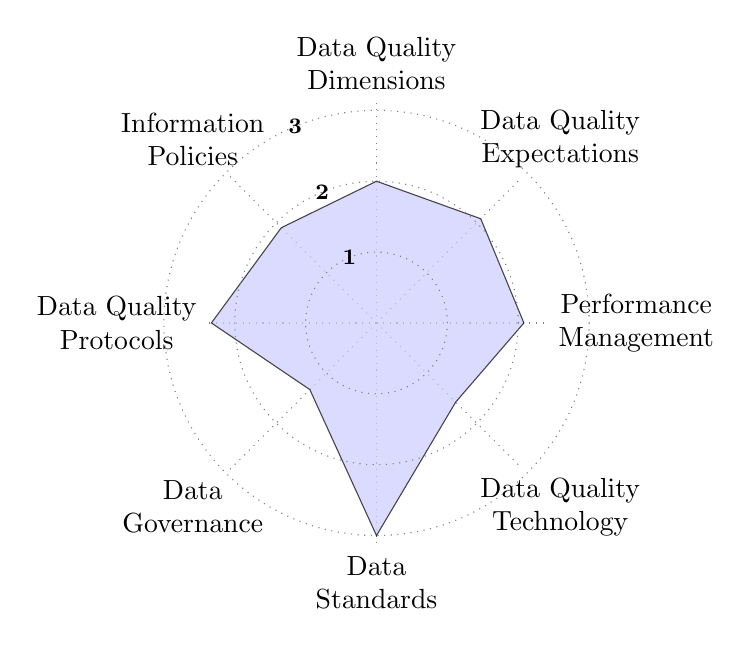
\begin{tikzpicture}[scale=0.3]
        % Define the origin of the spider graph
        \coordinate (origin) at (0, 0);

        % Define the maturity levels and corresponding labels
        \foreach[count=\i] \radius/\label in {
            2.08/Data Quality \\ Expectations,
            2.00/Data Quality \\ Dimensions,
            1.90/Information \\ Policies,
            2.33/Data Quality \\ Protocols,
            1.33/Data \\ Governance,
            3.00/Data \\ Standards,
            1.58/Data Quality \\ Technology,
            2.08/Performance \\ Management}{
            \coordinate (\i) at (\i * 360 / 8: \radius * 3); % Scale radius by 3 for better visibility
            \node[align=center] (label) at (\i * 360 / 8: 11) {\normalsize\label}; % Place labels
            \draw[gray, dotted] (origin) -- (label); % Connect labels to the origin
        }

        % Draw the filled polygon connecting all points
        \draw [fill=blue!20, opacity=.7] (1)
                                    \foreach \i in {2,...,8}{-- (\i)} -- cycle;

        % Add the grid lines for reference
        \foreach \r in {1, 2, 3} {
            \draw [gray, dotted] (0, 0) circle (\r * 3);
        }

        % Add concentric circle labels
        % \node at (0, 0) {\footnotesize\textbf{0}};
        \node at (112.5:3) {\footnotesize\textbf{1}};
        \node at (112.5:6) {\footnotesize\textbf{2}};
        \node at (112.5:9) {\footnotesize\textbf{3}};
    \end{tikzpicture}
    \caption{Maturity Level Spider Graph}
    \label{fig:maturity-level-spider-graph}
\end{figure}

By targeting a level just above the current one, organizations can make gradual improvements without overwhelming the staff. This approach helps achieve data quality benefits step by step, with clear goals along the way. In the end, this method leads to more manageable and effective improvements in data quality \cite{loshin_dqi}.

\subsection{Recommendations}
Gaps between its current data quality and the target expectations through assessments or interviews is identified. These gaps show characteristics that are not yet implemented. Based on these gaps, recommendations are made to improve DQM using DQM activities from the DMBOK to reach one level above the current state.

\begin{table*}[h]
\caption{Mapping the gaps in DQM maturity levels to the activities outlined in DQM-DMBOK}
\label{tab:mapping}
\centering
\begin{tabular}{|p{2cm}|p{5cm}|p{5cm}|p{2cm}|}
\hline
\textbf{Data Quality Component} & \textbf{Characteristics} & \textbf{Gap According to Current Condition} & \textbf{DMBOK Activity} \\
\hline
Data Quality Expectations (target = 3) & "No data quality expectations have been documented" & This company lacks internal documents outlining data quality expectations and relies only on related regulations like POJK and SEOJK & 7.1 \\
\hline
Data Quality Expectations (target = 3) & "Expectations associated with intrinsic dimensions of data quality associated with data values can be articulated" & There are no expectations for the intrinsic dimensions of data quality related to data value & 7.1 \\
\hline
Data Quality Expectations (target = 3) & "Dimensions of data quality are identified and documented" & Data quality dimensions have not been identified and documented & 7.2 \\
\hline
Data Quality Dimensions & 2.00 & Repeatable & \\
\hline
Information Policies & 1.90 & Initial & \\
\hline
Data Quality Protocols & 2.33 & Repeatable & \\
\hline
Data Governance & 1.33 & Initial & \\
\hline
Data Standards & 3.00 & Managed & \\
\hline
Data Quality Technology & 1.58 & Initial & \\
\hline
Performance Management & 2.08 & Repeatable & \\
\hline
\multicolumn{2}{|l|}{\textbf{Average}} & \textbf{2.04} & \textbf{Repeatable} \\
\hline
\end{tabular}
\end{table*}


\section{Conclusions and Future Works}

\subsection{Conclusions}

The study's findings lead to the following conclusions:

\begin{enumerate}
    \item The results of measuring the maturity level at PT Bank XYZ using the Loshin and DMBOK method \cite{loshin_dqi}\cite{DAMA_2013} indicate that the organization is still at level two. Our study shows that PT Bank XYZ has good level of Data Standard but is lacking in other areas such as Data Quality Technology and Data Governance.
    
    \item \lipsum[1] \todo{tambah conclusion}
\end{enumerate}


\subsection{Limitations and Future works}

\lipsum[1] \todo{fill this}

\section*{ACKNOWLEDGMENT}


Hopefully this research will provide value and benefit to readers, despite any shortcomings in its writing. The author extends gratitude to everyone who has offered support and assistance in completing this paper.

% \section*{References}
\bibliographystyle{IEEEtran}
\bibliography{references}

\end{document}
